\chapter{Deep-Reinforcement Learning}
Our first attempt to solve the problem of a neural network playing minesweeper is with deep--reinforcement learning.
Techniques able to learn Atari games~\cite{mnih2013playing} with a high input complexity should be able to learn and play `simpler' games like Minesweeper.
First we introduce the concept of Reinforcement learning with the addition of Deep Reinforcement Learning.
Afterwards we present our approach, followed by our results and the problems we encountered.

\section{Background}
Reinforcement learning is used to learn an optimal policy for an agent in an environment by exploring the environment and getting rewards based on its performance.
The environment $\mathcal{E}$ can be regarded as a sequence of actions, states and rewards.
At every time--step the agent selects a legal action $a_t$ from a set of legal game actions. 
The goal of the agent is to maximize the future reward.
We use as the future reward, the standard future discounted reward
\begin{equation}
R_t := \sum_{t'=t}^T \gamma^{t'-t}r_{t'},
\end{equation}
where $\gamma$ is a discount factor per time--step, $r_t$ represents the change in the game score and $T$ is the time--step at which the game is terminated.
The optimal action--value function $Q^*\left(s,a\right)$ is defined as the maximum expected return that will be returned by following any strategy:
\begin{equation}
Q^*\left(s,a\right):= \max_\pi \mathbb{E} \left[ R_t|s_t=s\text{, }a_t=a\text{, } \pi\right]
\end{equation}
where $s$ is some sequence and $\pi$ is a policy mapping sequences to actions.
%TODO belmann intuition erklären??
The optimal action--value function is gained with the Bellman equation by maximizing the expected value of $r+\gamma Q^*\left(s',a'\right),$
\begin{equation}
Q^*\left(s,q\right)= \mathbb{E}_{s' \sim \mathcal{E}} \left[ r + \gamma \max_{a'} Q^*\left(s',a'\right)| s,a \right],
\end{equation}
where $Q^*\left(s,a\right)$ is the sequence $s'$ at the next time--step for all possible actions $a'$. 
The value is maximized by selecting the optimal action $a'$.
With the Bellman equation the basic idea of reinforcement learning is introduced with an iterative update:
\begin{equation}
Q_{i+1}\left(s,a\right)= \mathbb{E}\left[r+\gamma \max_{a'} Q_i\left(s,a\right)| s,a\right],
\end{equation} 
where we assume that the value iteration algorithm converges to the optimal action--value function, i.e. $Q_i \rightarrow Q^*\text{, for } i \rightarrow \infty$.

For easy problems with small dimensions for the possible state--action space the Q--function can easily be saved in a table.
This table is updated while learning and represents the Q--function for each possible pair.
The state space for Minesweeper is incredibly large, thus a direct representation as a table does not work.
Neural networks can be used to encode a Q--function in a compact way.

For a neural network we need a non--linear approximation, where $\theta$ are the weights of the Q--network.
The Q--network is trained to minimize a sequence of loss functions $L_i\left(\theta_i\right)$, which changes in every iteration $i$,
\begin{equation}
L_i\left(\theta_i\right)= \mathbb{E}_{s,a \sim \rho \left( \cdot \right)}\left[ \left( y_i - Q\left(s,a;\rho_i \right) \right)^2\right],
\end{equation}
where $yi$ is the target at the $i-th$ iteration,
\begin{equation}
y_i = \mathbb{E}_{s'\sim \mathcal{E}}\left[ r+ \gamma \max_{a'} Q\left( s',a'; \theta_{i-1}\right)| s,a\right],
\end{equation}
and $\rho\left(s,a\right)$ is a probability distribution over the sequences $s$ and actions $a$, that is also called the behavior distribution.
To optimize the loss function $L_i\left(\theta_i\right)$ the parameters from the previous iteration $\theta_{i-1}$ are held fixed. 
Therefore, the target depends on the weights of the network. 
So to optimize we differentiate the loss function with respect to the weights and get the gradient,
\begin{equation}
\nabla_{\theta_i} L_i\left(\theta_i\right)= \mathbb{E}_{s,a\sim\rho\left(\cdot\right);s'\sim \mathcal{E}} \left[ \left( r + \gamma \max_{a'}Q\left(s',a';\theta_{i-1}\right) -Q\left(s,a;\theta_i\right) \right)\nabla_{\theta_i}Q\left(s,a;\theta_i\right)\right].
\end{equation}
Instead of calculating the expectation the loss function is optimized by stochastic gradient descent.
We get the Q--learning algorithm if the weights are updated after every step and the expectation is replaced by samples from $\rho$ and $\mathcal{E}$ respectively.

In contrast to supervised learning the target function depends on the weights of the network.
As the states of a game are highly correlated the basic assumption that the data used for learning is independent of each other does not hold.
Thus a memory is introduced which is filled continuously while playing and sampled randomly for learning.
This removes the correlation between game states as much as possible.
The memory contains the state, its reward, action, and the next state.
This reduces overfitting which would occur if the network is directly learned while playing.

As a policy we use $\epsilon$--greedy which takes a random action with the probability $\epsilon$ and otherwise takes the optimal action from the neural network.

\section{Our approach}
The environment is the the minesweeper field represented as an integer array.
An unvisited field is represented through $-1$ and $0$ to $8$ represent the number of adjacent mines.
The number of possible actions is equal to the size of the field and its encoding is the linear index of the two--dimensional array.
For the field size $8 \times 8$ we have 64 actions to open a field and 64 actions to flag or unflag a field (if it is already flagged).
If the agent takes action $8$, the field $(1, 0)$ would be opened.
Taking the action $8+64$, the field $(1, 0)$ would be flagged.

The Deep Q--network is defined in python in the framework tensorflow~\cite{tensorflow2015-whitepaper} and our code is oriented on a tutorial for Deep Q--networks~\cite{SimpleReLe}.

The main problem with Minesweeper compared to for example the Atari games is that the input dimension can change.
A `beginner' game is $8 \times 8$ with $10$ mines, whereas an `advanced' game is $16 \times 16$ with $40$ mines.
This is a big problem as the network needs to be resized and retrained for each size.
For the first try we restrict ourselves to the `beginner' size.

The first thing we noticed is the problem of our input size.
For example the Atari games are $84 \times 84$, whereas our input is $8 \times 8$.
With this small input a `deep' network is just not possible as each layer decreases the input size if you do not add padding.
Padding would create a whole different kind of problem for the encoding.
Thus we could only use a small amount of convolution layers to not destroy any positional information in the input data.
We tried several different architectures, but the results were pretty underwhelming.
The agent was prone to get stuck and it learned to perform worse than a random agent.
The reason for this bad performance is the overestimation of Q--values due to the network.
While a evenly distributed overestimation would not be harmful for the training process, an overestimation in a subset of suboptimal actions results impairs the learning of the optimal policy.
This results in feedback loops leading to a stuck training process, as the suboptimal action is taken over and over again.

To improve the stability of the network during training a separate target network can be used.
This type of Reinforcement Learning is called Double Q--Learning~\cite{HasseltGS15}.
Instead of updating it every few steps, we update $\theta'$, the weights from the target network, slowly every step by trailing the weights $\theta$ from the main network with a factor $\tau$~\cite{lillicrap2015continuous}.
\begin{equation}
	\theta' \leftarrow \tau\theta + (1-\tau)\theta' \text{ with } \tau \ll 1
\end{equation}
This results in a more stable training.
To reduce the overestimating of the Q--values, the estimation of the Q--value is decoupled from the action choice.
The primary network network chooses the action and the Q--value from the target, more stable, network is used.
\begin{equation}
	Q'(s, a) = r + \gamma Q(s', \arg\max_a(Q(s', a, \theta), \theta')) 
\end{equation}
This improves the stability of the training.

\section{Results}
As stated above we started with a `beginner' sized field $8 \times 8$.
To test the ability of our network to learn anything we started with one mine at a fixed position.
Figure~\ref{fig:fixed_mine} shows the average reward over a $100$ games each.
The reward for winning a game is $100$, which is the average reward after about a $1000$ played games.

\begin{figure}
	\centering
	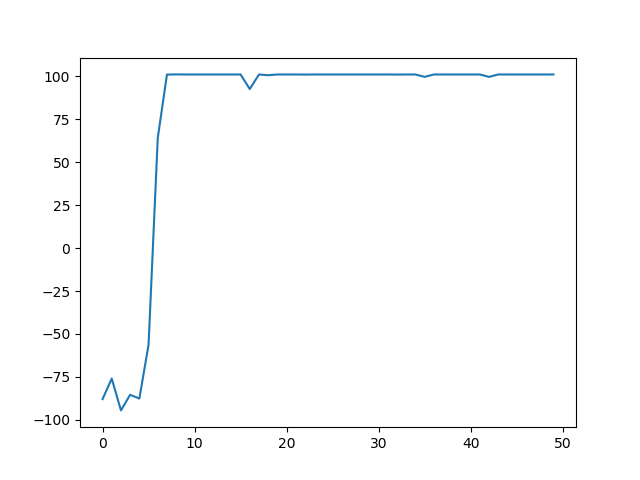
\includegraphics[width=\textwidth]{images/fixed_mine_position.png}
	\caption{Plot for the average reward during training with a fixed mine. The size is $8 \times 8$ and the agent learns to open the field and after that flags the mine. As can be seen, the agent learns it for the fixed mine.}
	\label{fig:fixed_mine}
\end{figure}

To increase the difficulty we randomized the position of the fixed mine.
Unfortunately the network was unable to flag the mine after it opened the first field.
The average reward of an exemplary game can be seen in Figure~\ref{fig:random_mine}.
The increase in average reward is due to the network minimizing its losses.
It just flagged or unflagged the same field over and over again.
At this moment we thought about the use of flags and came as already stated in the Introduction, that flagging as an action for a computer player does not make sense.
A human can use flags to mark mines as a reminder but for winning the game only all none--mine fields need to be opened.
To reduce the amount of possible actions for the agent we removed the flag actions, further reducing the possibility of unflagging/flagging a field forever.

\begin{figure}
	\centering
	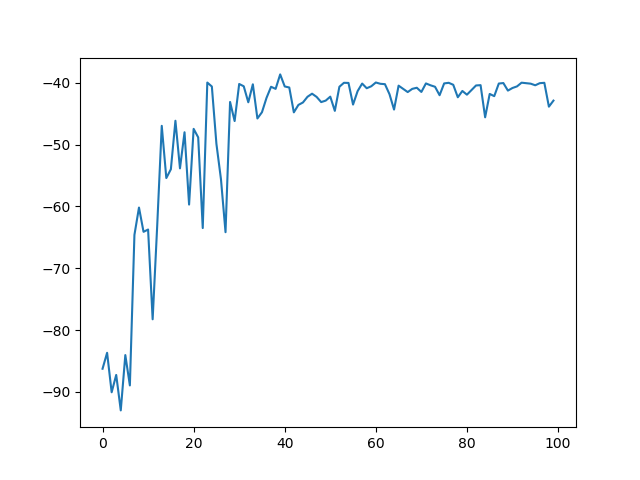
\includegraphics[width=\textwidth]{images/random_mine_position.png}
	\caption{Plot for the average reward during training with a random mine. The size is $8 \times 8$ and the agent tries to learn to open any field and after that flags the mine. The agent gets stuck during learning.}
	\label{fig:random_mine}
\end{figure}

The problem with removing the flagging option are the slightly different win conditions.
Previously the agent could only win the game by opening all fields and flagging all mines.
Without the flagging option the agent wins the game by opening all fields except the ones with mines beneath.
With just one mine, the agent always wins the game except by opening the field with the mine beneath in the first move.

To reduce the complexity of the agent and also reduce the time needed for simulations we reduced the size of the field to $5 \times 5$.
This was the smallest we could get while still using convolution layers, that made at least some sense.
Additionally we introduced the previously explained concept of Double Deep Q--networks to improve the training stability.

The result of one of the runs can be seen in Figure~\ref*{fig:DDQN_still_unstable}.
The negative reward from up to $-400$ stems from the changed reward policy.
Opening an already opened field is penalized by a reward of $-20$.
Winning, Losing and opening a field is rewarded with $100$, $-100$ and $1$ respectively.
The second graph shows the percentage of wining, losing or not finishing a game.
Games are aborted after a specific number of moves, in this case 25 to allow the agent to open every field and to take some useless actions.
The $20\%$ lose rate is based on our game model, as the mines are already positioned before the first move.
Thus the agent directly loses $\#mines/\#fields$ games at the first move.
But even with the additional stability measures from the Double DQN the training gets stuck after about $100000$ episodes.
We tried multiple parameter changes but even for a $5 \times 5$ field the computational time needed is immense.

\begin{figure}
	\centering
	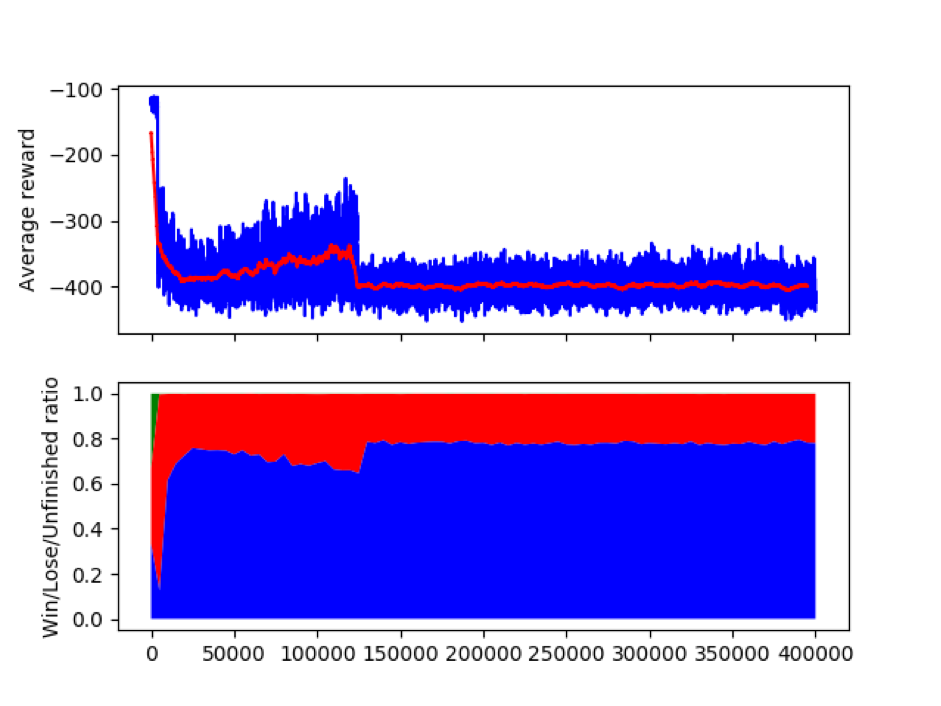
\includegraphics[width=\textwidth]{images/CNN-2nd-Plot.png}
	\caption{Exemplary plot for the reward and win/lose/unfinished rates during training of a Double DQN. The $20\%$ lose rate is due to the agent hitting a mine on the first move. Unfortunately the training is still unstable.}
	\label{fig:DDQN_still_unstable}
\end{figure}


